\documentclass[jkps,preprint,fleqn,showpacs,showkeys]{revtex4}

\usepackage{graphicx}
\usepackage{amssymb}
\usepackage{amsmath}
\usepackage{bm}
\usepackage{lineno}
\usepackage{xspace}
\usepackage{cleveref}

%% $Id: commands.tex 934 2013-06-19 20:56:45Z mfloris $

\newcommand{\pp}{\mbox{$pp$}\xspace}
\newcommand{\pythia}{\textsc{Pythia8}\xspace}
\newcommand{\deta}{\mbox{$\Delta\eta$}\xspace}
\newcommand{\pt}{\mbox{$p_{T}$}\xspace}
\newcommand{\pT}{\mbox{$p_{T}$}\xspace}

\newcommand{\mrm}[1]{\mathrm{#1}}
\newcommand{\mrmo}[1]{\mathrm{\overline{#1}}}
\newcommand{\bsb}[1]{\boldsymbol{#1}}
\newcommand{\circit}{\item[$\circ$]}

\newcommand{\ITS}          {\rm{ITS}}
\newcommand{\TOF}          {\rm{TOF}}
\newcommand{\ZDC}          {\rm{ZDC}}
\newcommand{\ZDCs}         {\rm{ZDCs}}
\newcommand{\ZNA}          {\rm{ZNA}}
\newcommand{\ZNC}          {\rm{ZNC}}
\newcommand{\SPD}          {\rm{SPD}}
\newcommand{\SDD}          {\rm{SDD}}
\newcommand{\SSD}          {\rm{SSD}}
\newcommand{\TPC}          {\rm{TPC}}
\newcommand{\VZERO}        {\rm{VZERO}}
\newcommand{\VZEROA}       {\rm{VZERO-A}}
\newcommand{\VZEROC}       {\rm{VZERO-C}}
\newcommand{\pip}          {$\pi^{+}$}
\newcommand{\pim}          {$\pi^{-}$}
\newcommand{\kap}          {K$^{+}$}
\newcommand{\kam}          {K$^{-}$}
\newcommand{\pbar}         {$\rm\overline{p}$}
\newcommand{\kzero}        {\ensuremath{{\rm K}^{0}_{S}}}
\newcommand{\kstar}        {\ensuremath{{\rm K}^{*}}}
\newcommand{\He}           {\ensuremath{^{3}{\rm He}}}
\newcommand{\LH}           {\ensuremath{^{3}_{\Lambda}{\rm H}}}
\newcommand{\vzero}        {\ensuremath{{\rm V}^0}}
\newcommand{\lmb}          {\ensuremath{\Lambda}}
\newcommand{\almb}         {\ensuremath{\bar{\Lambda}}}
\newcommand{\allpart}      {$\pi^{\pm}$, K$^{\pm}$, \kzero, p(\pbar) and \lmb(\almb)}
\newcommand{\allpi}        {$\pi^{\pm}$}
\newcommand{\allk}         {K$^{\pm}$}
\newcommand{\allp}         {p(\pbar)}
\newcommand{\alllmb}       {\lmb(\almb)}
\newcommand{\degree}       {$^{\rm o}$}
\newcommand{\dg}           {\mbox{$^\circ$}}
\newcommand{\dedx}         {\ensuremath{\mathrm{d}E/\mathrm{d}x}}
\newcommand{\dndy}         {d$N$/d$y$}
\newcommand {\ee}            {\mbox{e$^+$e$^-$}}
%\newcommand{\pp}           {pp}
\newcommand{\ppbar}        {\mbox{$\mathrm {p\overline{p}}$}}
\newcommand{\PbPb}         {\mbox{Pb--Pb}}
\newcommand{\pPb}          {\mbox{p--Pb}}
\newcommand{\AuAu}         {\mbox{Au--Au}}
\newcommand{\pseudorap}    {\mbox{$\left | \eta \right | $}}
\newcommand{\dNdeta}       {\ensuremath{\mathrm{d}N_\mathrm{ch}/\mathrm{d}\eta}}
\newcommand{\dNdy}         {\ensuremath{\mathrm{d}N/\mathrm{d}y}}
\newcommand{\dNdptdy}      {\ensuremath{\mathrm{d}N/{\rm d}\pt\mathrm{d}y}}
\newcommand{\dNdyst}       {\ensuremath{\sqrt{\frac{dN_\pi/dy}{s_T}}}}
\newcommand{\dNdetatr}     {\mathrm{d}N_\mathrm{tracklets}/\mathrm{d}\eta}
\newcommand{\dNdetar}[1]   {\mathrm{d}N_\mathrm{ch}/\mathrm{d}\eta\left.\right|_{|\eta|<#1}}
\newcommand{\lum}          {\, \mbox{${\rm cm}^{-2} {\rm s}^{-1}$}}
\newcommand{\barn}         {\, \mbox{${\rm barn}$}}
\newcommand{\m}            {\, \mbox{${\rm m}$}}
\newcommand{\ncls}         {\ensuremath{N_{cls}}}
\newcommand{\nsigma}       {\ensuremath{n\sigma}}
\newcommand{\dcaxy}        {\ensuremath{{\rm DCA}_{xy}}}
\newcommand{\dcaz}         {\ensuremath{{\rm DCA}_{z}}}
\newcommand{\EcrossB}      {E$\times$B}%{\ensuremath{{\rm E}\times{\rm B}}}
\newcommand{\bb}           {Bethe-Bloch}
\newcommand{\s}            {\ensuremath{\sqrt{s}}}

\newcommand{\hlab}         {\ensuremath{\eta_{\rm lab}}}
\newcommand{\ynn}         {\ensuremath{y_{\rm NN}}}
\newcommand{\ycms}         {\ensuremath{y_{\rm CMS}}}
\newcommand{\ylab}         {\ensuremath{y_{\rm lab}}}
\newcommand{\ppi}          {\ensuremath{{\rm p}/\pi}}
\newcommand{\kpi}          {\ensuremath{{\rm K}/\pi}}
\newcommand{\lpi}          {\ensuremath{{\rm \Lambda}/\pi}}
%\newcommand{\ppi}          {\ensuremath{(\pi^+ + \pi^-)/({\rm K}^+ + {\rm K}^-)}}
%\newcommand{\kpi}          {\ensuremath{({\rm p} + {\rm \bar p})/({\rm K}^+ + {\rm K}^-)}}
\newcommand{\mt}           {\ensuremath{m_{\rm T}}}
\newcommand{\snn}          {\ensuremath{\sqrt{s_{\rm NN}}}}
\newcommand{\snnbf}        {\ensuremath{\mathbf{{\sqrt{s_{\mathbf NN}}}}}}
\newcommand{\sonly}        {\ensuremath{\sqrt{s}}}
\newcommand{\Npart}        {\ensuremath{N_\mathrm{part}}}
\newcommand{\avNpart}      {\ensuremath{\langle N_\mathrm{part} \rangle}}
\newcommand{\avNpartdata}  {\ensuremath{\langle N_\mathrm{part}^{\rm data} \rangle}}
\newcommand{\Ncoll}        {\ensuremath{N_\mathrm{coll}}}
\newcommand{\Dnpart}       {\ensuremath{D\left(\Npart\right)}}
\newcommand{\DnpartExp}    {\ensuremath{D_{\rm exp}\left(\Npart\right)}}
\newcommand{\dNdetapt}     {\ensuremath{\dNdeta\,/\left(0.5\Npart\right)}}
\newcommand{\dNdetaptr}[1] {\ensuremath{\dNdetar{#1}\,/\left(0.5\Npart\right)}}
\newcommand{\dNdetape}     {\left(\ensuremath{\dNdeta\right)/\left(\avNpart/2\right)}}
\newcommand{\dNdetaper}[1] {\ensuremath{\dNdetar{#1}\,/\left(\avNpart/2\right)}}
\newcommand{\dndydpt}      {\ensuremath{{\rm d}^2N/({\rm d}y {\rm d}p_{\rm t})}}
\newcommand{\abs}[1]       {\ensuremath{\left|#1\right|}}
\newcommand{\signn}        {\ensuremath{\sigma^{\rm inel.}_{\rm NN}}}
\newcommand{\vz}           {\ensuremath{V_{z}}}
\newcommand{\Tfo}          {\ensuremath{{T}_{\rm kin}}}
\newcommand{\Tch}          {\ensuremath{{T}_{\rm ch}}}
\newcommand{\bT}           {\ensuremath{\beta_{\rm T}}}
\newcommand{\avbT}         {\ensuremath{\left< \beta_{\rm T}\right>}}
\newcommand{\avpT}         {\ensuremath{\left< \pt \right>}}
\newcommand{\muB}          {\ensuremath{\mu_{B}}}
\newcommand{\stat}         {({\it stat.})}
\newcommand{\syst}         {({\it sys.})}
\newcommand{\Fig}[1]       {Fig.~\ref{#1}}
\newcommand{\Figure}[1]    {Figure~\ref{#1}}
%\newcommand{\Ref}[1]       {Ref.~\cite{#1}}
%\newcommand{\green}[1]     {\textcolor{green}{#1}}
%\newcommand{\blue}[1]      {\textcolor{blue}{#1}}
%\newcommand{\red}[1]       {\textcolor{red}{#1}}
%\newcommand{\white}[1]     {\textcolor{white}{#1}}
\newcommand{\gevc}         {\ensuremath{{\rm GeV}/c}}
\newcommand{\mevc}         {\ensuremath{{\rm MeV}/c}}
\newcommand{\gs}           {\ensuremath{\gamma_{s}}}
\newcommand{\gq}           {\ensuremath{\gamma_{q}}}
\newcommand{\gc}           {\ensuremath{\gamma_{c}}}
\newcommand{\chindf}       {\ensuremath{\chi^{2}/{\rm NDF}}}
\newcommand{\avg}[1]       {\ensuremath{\left\langle#1\right\rangle}}
\newcommand{\etalab}       {\ensuremath{\eta_{{\rm lab}}}}
\newcommand {\gammas}			{\ensuremath{\gamma_{\mathrm{s}}}}
\newcommand{\DNDETAINEL}{5.31~$\pm$~0.18\xspace}
\newcommand{\DNDETAINELGTZERO}{6.46~$\pm$~0.19\xspace}
\newcommand{\DNDETAINELGTZEROONE}{6.61~$\pm$~0.20\xspace}
\newcommand{\inelgtzero}{INEL$>$0\xspace}
\newcommand{\average}[1]{\ensuremath{\langle #1 \rangle}\xspace}
\newcommand{\mpt}        {\ensuremath{\langle\pt\rangle}\xspace}
\newcommand{\nch}        {\ensuremath{N_\mathrm{ch}}\xspace}
\newcommand{\mnch}      {\ensuremath{\langle\nch\rangle}\xspace}
\newcommand{\nchacc}        {\ensuremath{N_\mathrm{ch}^\mathrm{acc}}\xspace}
\newcommand{\mnchacc}      {\ensuremath{\langle\nchacc\rangle}\xspace}
\newcommand{\inelg}     {\ensuremath{\mathrm{INEL}_{>0}}}



\newcommand{\dndeta}{\ensuremath{{\rm d}N_{\rm ch}/{\rm d}\eta}\xspace}
\newcommand{\dndpt}{\ensuremath{{\rm d}N_{\rm ch}/{\rm d}\pt}\xspace}
\newcommand{\etaless}[1]{\ensuremath{\left|\eta\right| < #1}\xspace}
\newcommand{\dndetaless}[1]{\ensuremath{{\rm d}N_{\rm ch}/{\rm d}\eta|_{\etaless{#1}}}\xspace}
\newcommand{\avdndeta}{\ensuremath{\langle \dndeta \rangle}}
\newcommand{\zvtx}{\ensuremath{z_\mathrm{vtx}}}


\newcommand{\pythiam}{\ensuremath{\mathrm{PYTHIA}\,8\,\mathrm{tune}}{\text -}4c}
\newcommand{\pythiashoving}{{\ensuremath{\mathrm{PYTHIA}\,8~\mathrm{String}~}}\ensuremath{\mathrm{Shoving}}}
\newcommand{\epos}{{\ensuremath{\mathrm{EPOS}\,~\mathrm{LHC}}}}
%\newcommand{\pythiashoving}{\ensuremath{\mathrm{PYTHIA}\,8~\mathrm{String}~}\linenomath{-}\ensuremath{\mathrm{Shoving}}}
\newcommand{\pttrig}{\ensuremath{p_\mathrm{T,\,trig}}}
\newcommand{\ptassoc}{\ensuremath{p_\mathrm{T,\,assoc}}}
\newcommand{\ptjet}{\ensuremath{p_\mathrm{T,\,Jet}}}
\newcommand{\ptlead}{\ensuremath{p_\mathrm{T,\,LP}}}
\newcommand{\pttrigassoc}{\ensuremath{p_\mathrm{T,\,trig\,(assoc)}}}









\renewcommand{\labelitemi} {$-$}
%==========================================================%
%%% inline warnings for internal discussion
%\newcommand{\warn}[1]      {\textbf{\textcolor{red}{[#1]}}}
\newcommand{\warn}[1]      {{\small\textbf{\textcolor{red}{(!\footnote{\textbf{(!)}~#1})}}}}
\newcommand{\warnin}[1]         {\textit{\textcolor{red}{(#1)}}}
%\newcommand{\warn}[1]      {#1}
%\newcommand{\warn}[1]      {{\small\textbf{(!\footnote{\textbf{(!)}~#1})}}\marginpar{\textbf{---}}}
\newcommand{\todo}[1]      {\textbf{\textcolor{red}{[TODO: #1]}}}
%%% fake numbers
\newcommand{\fake}[1]      {\textbf{\textcolor{red}{#1}}}
%\newcommand{\fake}[1]      {#1}
\newcommand{\final}[1]     {\textbf{\textcolor{blue}{#1}}}
\newcommand{\prelim}[1]    {\textbf{\textcolor{magenta}{#1}}}
\renewcommand{\mod}[1]       {\textbf{\textcolor{red}{#1}}}


\newcommand{\XGB}{XGBoost}

\begin{document}
\setcounter{page}{0}
\title[]{ A Monte Carlo based new sampling calorimeter toward the measurement of $\gamma$ incident angle }

\author{YoungJun \surname{Kim}}
\affiliation{Department of Physics, Korea University, Seoul 02841}
\author{Junlee \surname{Kim}}
\email{junlee.kim@cern.ch}
\author{Eun-Joo \surname{Kim}}
\affiliation{Department of Physics education, Jeonbuk National University, Jeonju 54896}
\author{GeiYoub  \surname{Lim}}
\affiliation{IPNS/KEK Tsukuba, Japan 305-0801}

%\date[]{Received 6 August 2007}

\begin{abstract}
SHORT MOTIVATION HERE. 
We present the studies on Monte Carlo based detector configuration to measure the incident angle of the $\gamma$. The Geant4 and the $\XGB$ packages are used to simulate interactions of electromagnetic showers with detector materials and to reconstruct the incident angle with the machine learning method. The sandwich-type sampling calorimeter is configured with 5-mm-thick scintillator strips and 1-mm-thick lead plates. The sampling fraction and the Moliere radius of the detector are xxx and xxx, respectively. We find that the configuration with 15-mm-wide scintillator strips is found to provide xxx resolution and the front part of the detector as much as 4.6-radiation-length thickness provides the same resolution with xxx inefficiency.
\end{abstract}


%\pacs{68.37.Ef, 82.20.-w, 68.43.-h}
%\keywords{String shoving, Collectivity, $pp$ collision}
\maketitle

\section{Motivation}
\label{sec:mot}
Electromagnetic calorimeter (EM-Cal) has played an important role in nuclear and particle physics especially to detect photon[]. The most important property of the detector is good energy and timing resolution, and various crystals has been developed for the purpose[]. On the other hand, the sampling calorimeter consisting of alternating converter generating shower particles and counter measuring energy deposit of the shower particles tends to replace the crystal calorimeter in large-scale high energy experiment[].

Due to a fluctuation of energy deposit in the converter, sampling fluctuation, the sampling calorimeter suffers poor energy resolution. This fluctuation becomes not so important for high energy photons owing to large number of shower particles. When we use a plastic scintillator as a counter, we can fabricate a large scale of calorimeter with relatively low cost.  
There are many efforts to develop new types of calorimeter and a fine-segmented sampling calorimeter is in the line[]. 

The sampling calorimeter enable us to measure not only energy but also incident angle of photon. Considering a stochastic process in shower generation, there is a certain limitation of detection resolution. Also, the effect of sampling fluctuation is matter in medium energy photons in range 100 MeV to few GeV photons. Even though these drawbacks, there is an experiment to have quite strong motivation on developing the calorimeter able to measure incident angle.

KOTO experiment, being performed at the J-PARC in Japan, aims at searching for the $K_L \rightarrow \pi^0 \nu \bar{\nu}$ decay.  This decay is very clean in theoretical calculation[] and large potential to access the new physics beyond the Standard Model[]. However, current experimental sensitivity is still far from the SM expectation[] mainly due to its extremely small branching fraction and very weak kinematic condition to define a signature of the decay. 

Considering negligible detection efficiency on neutrinos, the $K_L \rightarrow \pi^0 \nu \bar{\nu}$ decay is defined as an event existing only single $\pi^0$ in the final sate which is reconstructed by detecting two photons generated from prompt decay of the $\pi^0$. The KOTO utilizes un-doped cesium iodide (CsI) crystals as an EM-Cal to measure the photons. An hermetic detector system surrounding decay region confirms that there is no any particles accompanying the two photons[]. 

In reality, energies and positions of two photons measured at the EM-Cal are not enough to reconstruct the $\pi^0$, and we need an assumption that they are generated from the $\pi^0$ decaying at beam axis. This reconstruction is totally failed in case the assumption is not correct any more, but there is no information to figure out, unfortunately. 
 In addition to the current reconstruction of $\pi^0$, we can extract its decay position independently with the angle measurement. By requiring a consistency between two vertices reconstructed from different observables, we can select genuine single $\pi^0$ decay rejecting various kinds of wrong pair of photons such as odd-pairing of $K_L \rightarrow \pi^0 \pi^0$ decays, neutron induced two clusters, and so on. It also enable us to remove $\pi^0$ and $\eta$ decays produced by halo neutrons because they occur far from the beam axis. We can expect similar rejection against $K_L \rightarrow \gamma \gamma$ decays when the $K_L$ deviate form the beam center due to scattering. 

For the angle measurement of photon, we should get an information about the spatial profile of shower particles generated in the electromagnetic calorimeter. This will be realized by recording energy deposit to the cell of detector separately, which are finely segmented in three dimensions. 
A sampling calorimeter consisting of alternating lead sheet and strips of plastic scintillator could be a good candidate of the calorimeter as describe in this paper.



\section{method}
\label{sec:ana}
\subsection{Detector construction}
We constructed a prototype sampling electromagnetic calorimeter with alternative stacking of thin Pb sheets and scintillator strips. A Pb sheet has a dimension of 50 cm (w) $\times$ 50 cm (l) $\times$ 1 mm (t). And a single layer of scintillator plate consists of 25 long scintillator segments, and each segment has a dimension of 2 cm (w) $\times$ 50 cm (l) $\times$ 5 mm (t). The full geometry consists of 105 layers  which is corresponding to 20 $X_0$. 



\subsection{XGBOOST: A toolkit for machine learning}
\label{sec:anaML}
Among many packages for machine learning in the high energy physics area~\cite{ATLAS:2020iwa} is the $\XGB$, supporting a scalable tree boosting system~\cite{xgboost:2016}. The $\XGB$ package is used to reconstruct the incident angle of incident $\gamma$ particles with deposit energies, which is mainly from the secondary particles of the EM shower, in the each channel. The $\XGB$ requires that the number of input data is identical, which is defined as the number of channels in this paper. For the $\XGB$ to reconstruct the angle, the training procedure for the $\XGB$ needs to be preceded. The training procedure helps the $\XGB$ study how $\gamma$ interacts with the detector and deposits the energy to the each channel with respect to the incident angle for a given $\gamma$ energy. Input data, deposit energies for whole channels, are obtained from the calculation of the EM shower in the detector simulated by the Geant4 package. Simulations are done with the uniform incident polar angle ($\theta$) distribution from 0 to 50 degree and the uniform azimuthal angle ($\varphi$) from 0 to 360 degree for the training, which makes the $\XGB$ possible to reconstruct events having 0~$<\theta<$~50~degree and 0~$<\varphi<$~360~degree. The reconstruction of $\theta$ by the $\XGB$, completing the training procedure, is tested with the fixed $\theta$ and uniform $\varphi$ from 0 to 360 degree.

\section{Results}
\label{sec:res}

\subsection{Detector property}

\subsection{Parameterization for machine learning setting}
The configuration of the $\XGB$ can be defined with five parameters, described in Tab.~\ref{tab:XgbPar}. The parameters are selected as one providing better angular resolution. It is found that the Max. depth mostly affects the angular resolution, and the resolution is not enhanced for Max. depth~$>$~15 any more. It is also worth mentioning that the N\_estimators larger than 1000 does not provide better resolution with the Max. depth~=~15. The angular resolution of the reconstruction is defined as the standard deviation of Gaussian function, whose parameters are evaluated by fitting the reconstructed angle distribution. Figure~\ref{fig:angle_reco_def} shows the reconstructed $\theta$ distribution with respect to each incident $\theta$ with described training parameters. The angular resolution for all $\theta$ is estimated to be about 1.3~degree.

\begin{figure}[!hbt]
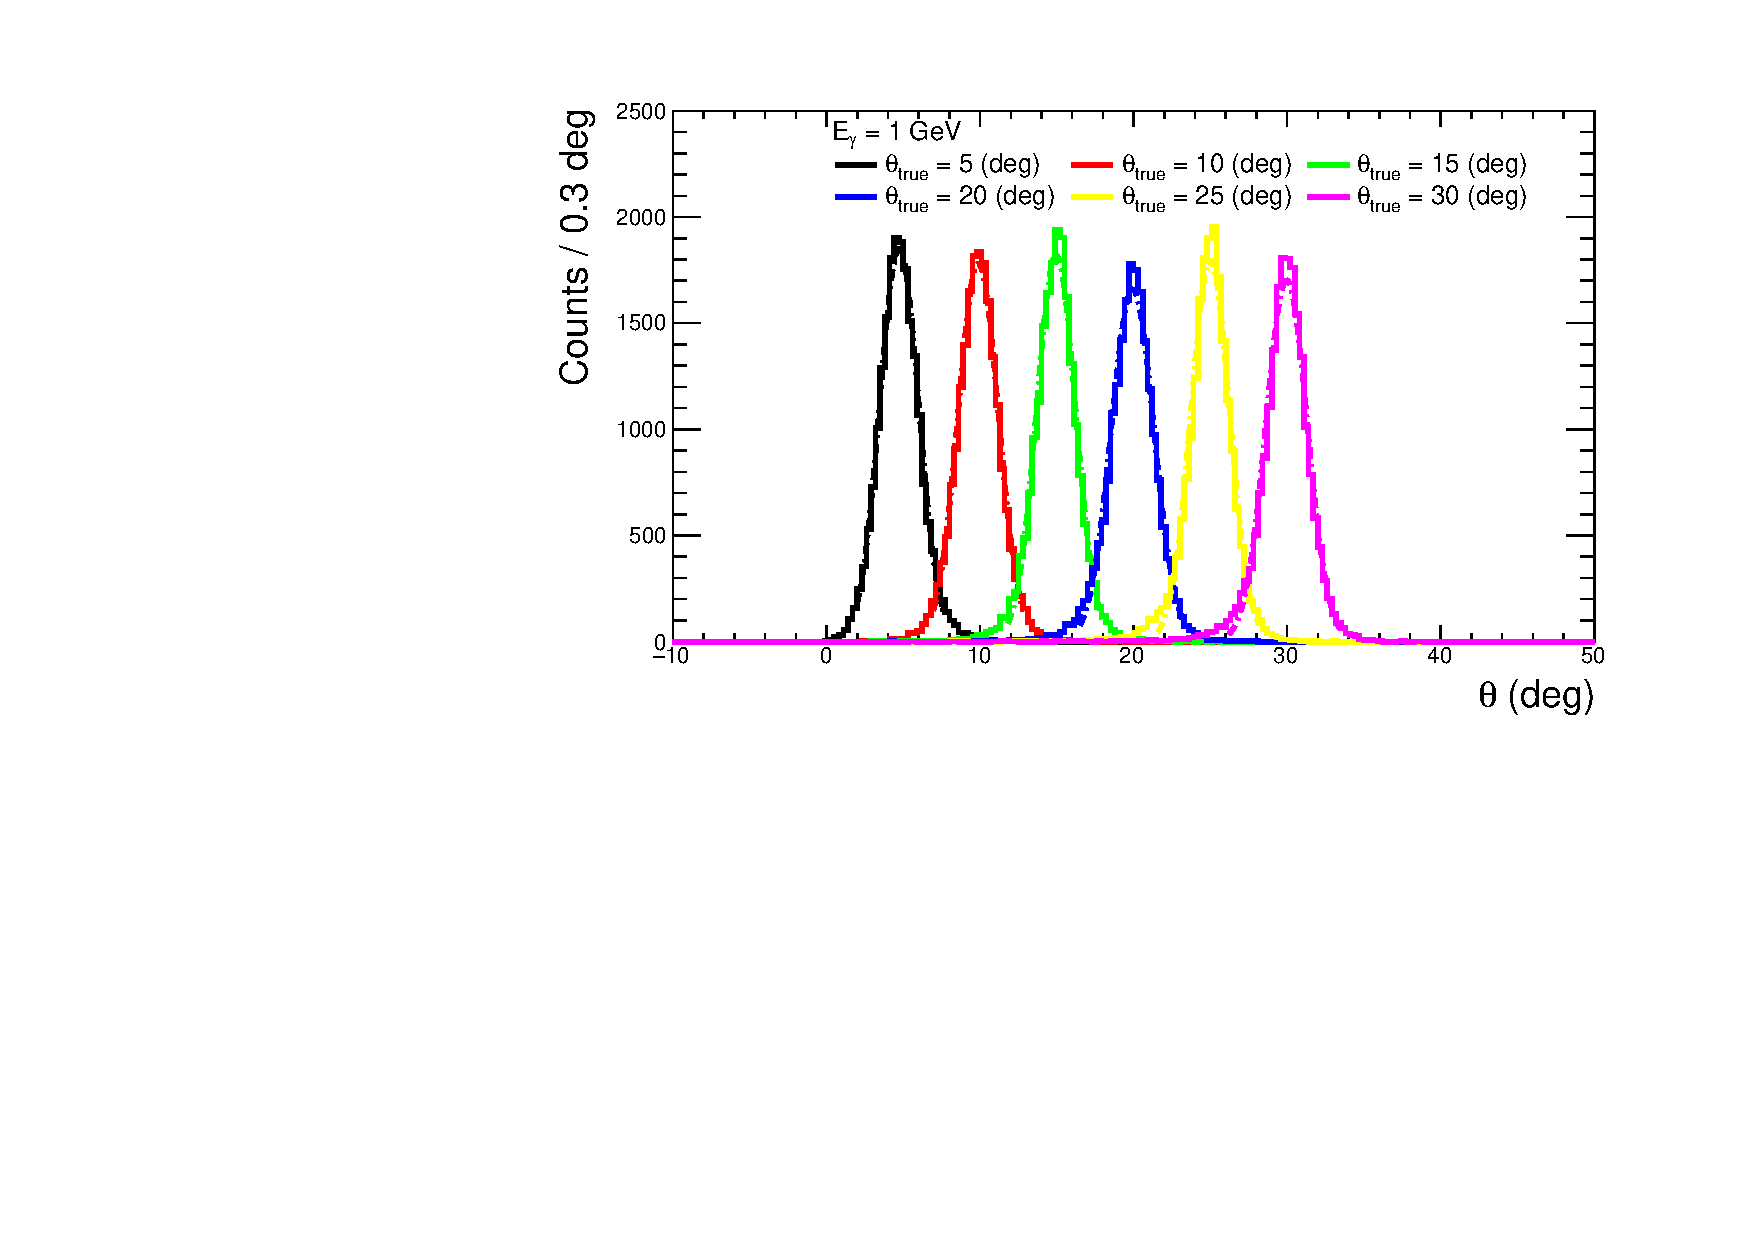
\includegraphics[width=0.89\textwidth]{figures/Fig1_reco_def.pdf}
\caption{ (Color online) Reconstructed $\theta$ with respect to each true incident $\theta$ dotted lines denote each Gaussian function fitting the reconstructed $\theta$ distribution. The standard deviation of all Gaussian functions are estimated to be about 1.3 degree.}
\label{fig:angle_reco_def}
\end{figure}

\begin{table}[hbt!]
\centering
\caption{Parameterization of the $\XGB$}
\begin{tabular}{ccc}
\hline 
Parameter & Function & Suggested value \\ \hline 
N\_estimators & The number of decision trees & 1000 \\  
Max. depth & Possible maximum depth of tree structure & 15 \\ 
Subsample & Fraction of total data used for a single decision & 1 \\ 
Learning rate & Step length for calculation & 0.08 \\ 
Gamma & Requirement on minimum loss function & 0 \\ 
\hline
\end{tabular}
\label{tab:XgbPar}
\end{table}

\subsection{Detector dimension}
\begin{figure}[!hbt]
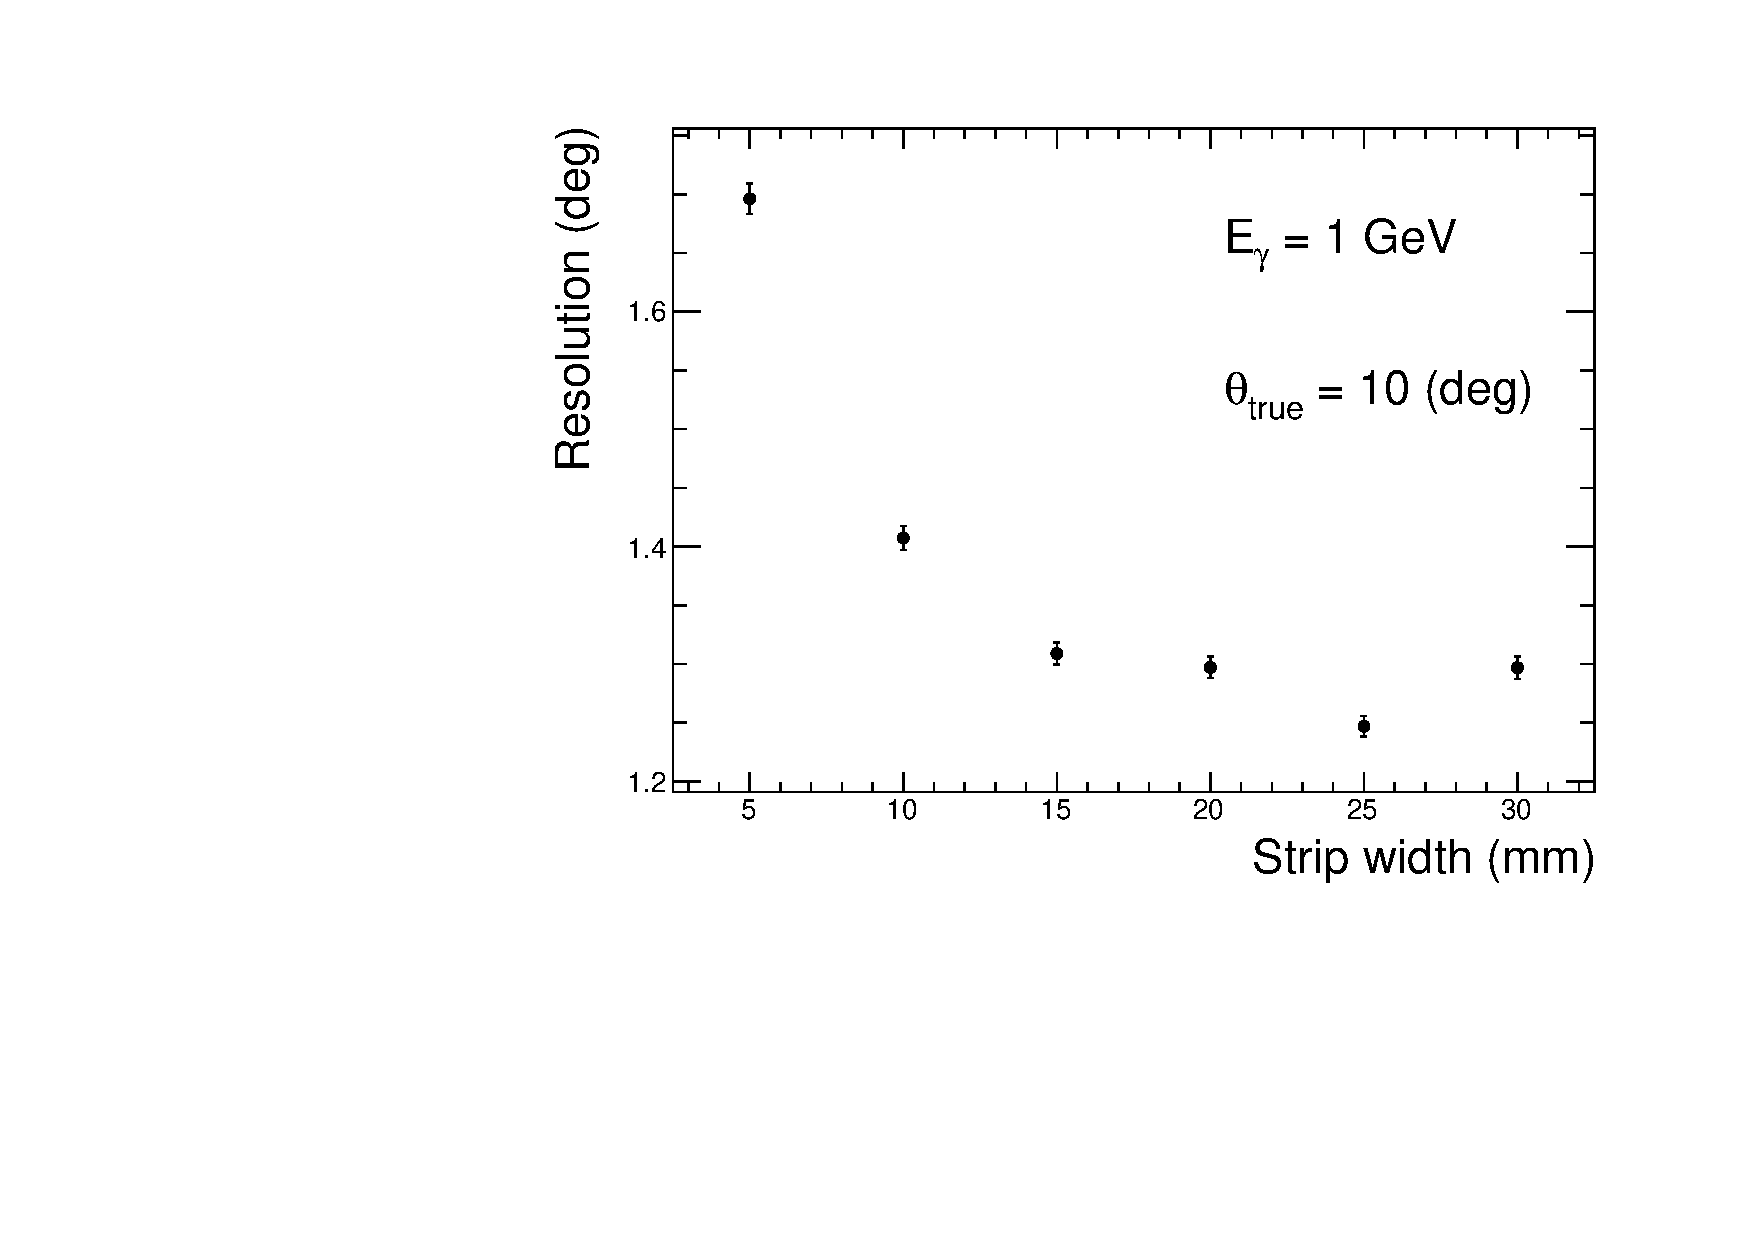
\includegraphics[width=0.58\textwidth]{figures/Fig2_reco_Width_width.pdf}
\caption{ The angular resolution as a function of the scintillator strip width for 1 GeV $\gamma$. The incident angle for each simulation is fixed as 10 degree.  }
\label{fig:angle_reco_width}
\end{figure}

The performance of the detector is tested with different detector dimensions. Different geometries are simulated in the Geant4 package and corresponding training procedures are applied with the same number of training events as 100,000. Figure~\ref{fig:angle_reco_width} shows the angular resolution of the reconstruction as a function of the scintillator strip width with the 5-mm step. It if found that the configuration with 15-mm-wide strips provides better resolution than one with smaller strip widths, and the configuration with larger strip size than 15 mm does not provide improved resolution. Based on this, The width of the strip is determined to be 15 mm.

\begin{figure}[!hbt]
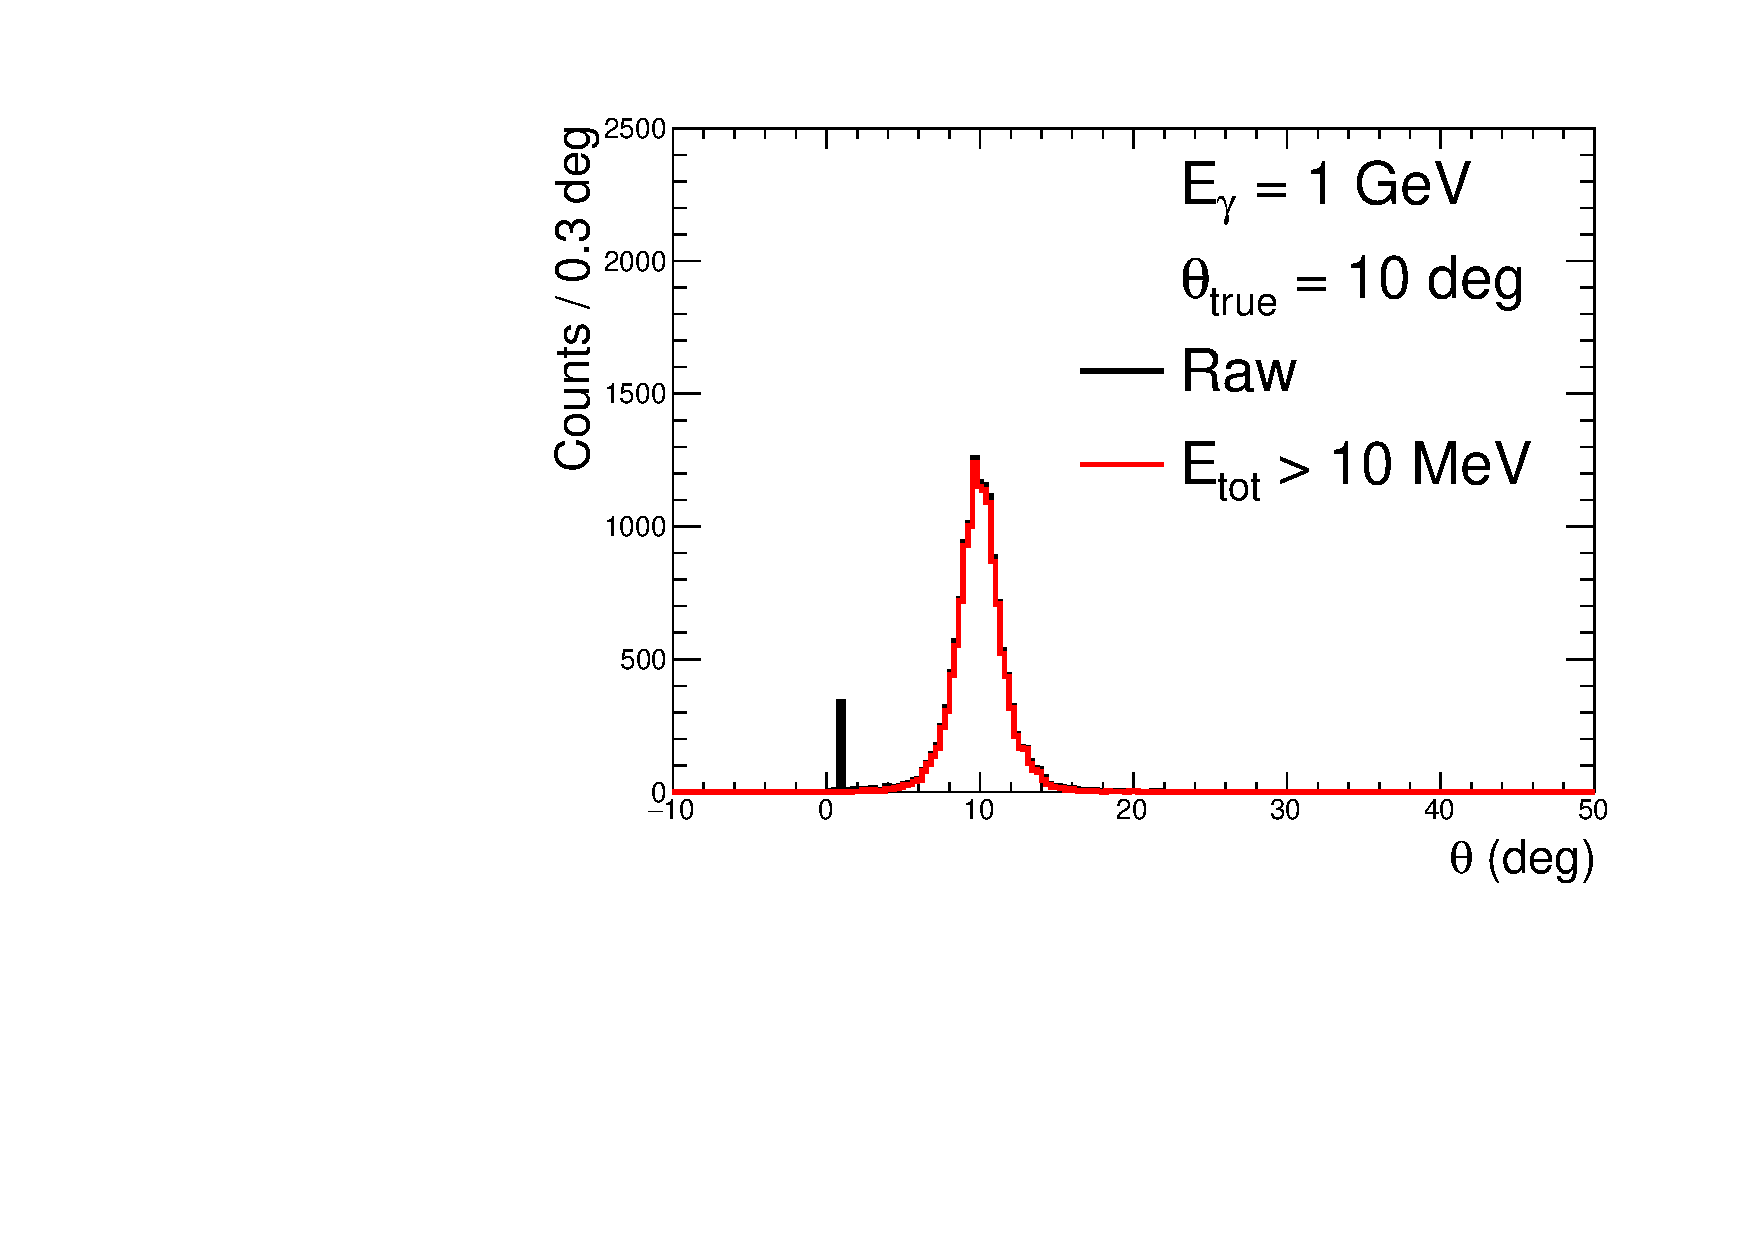
\includegraphics[width=0.48\textwidth]{figures/Fig3_reco_layer_hist.pdf}
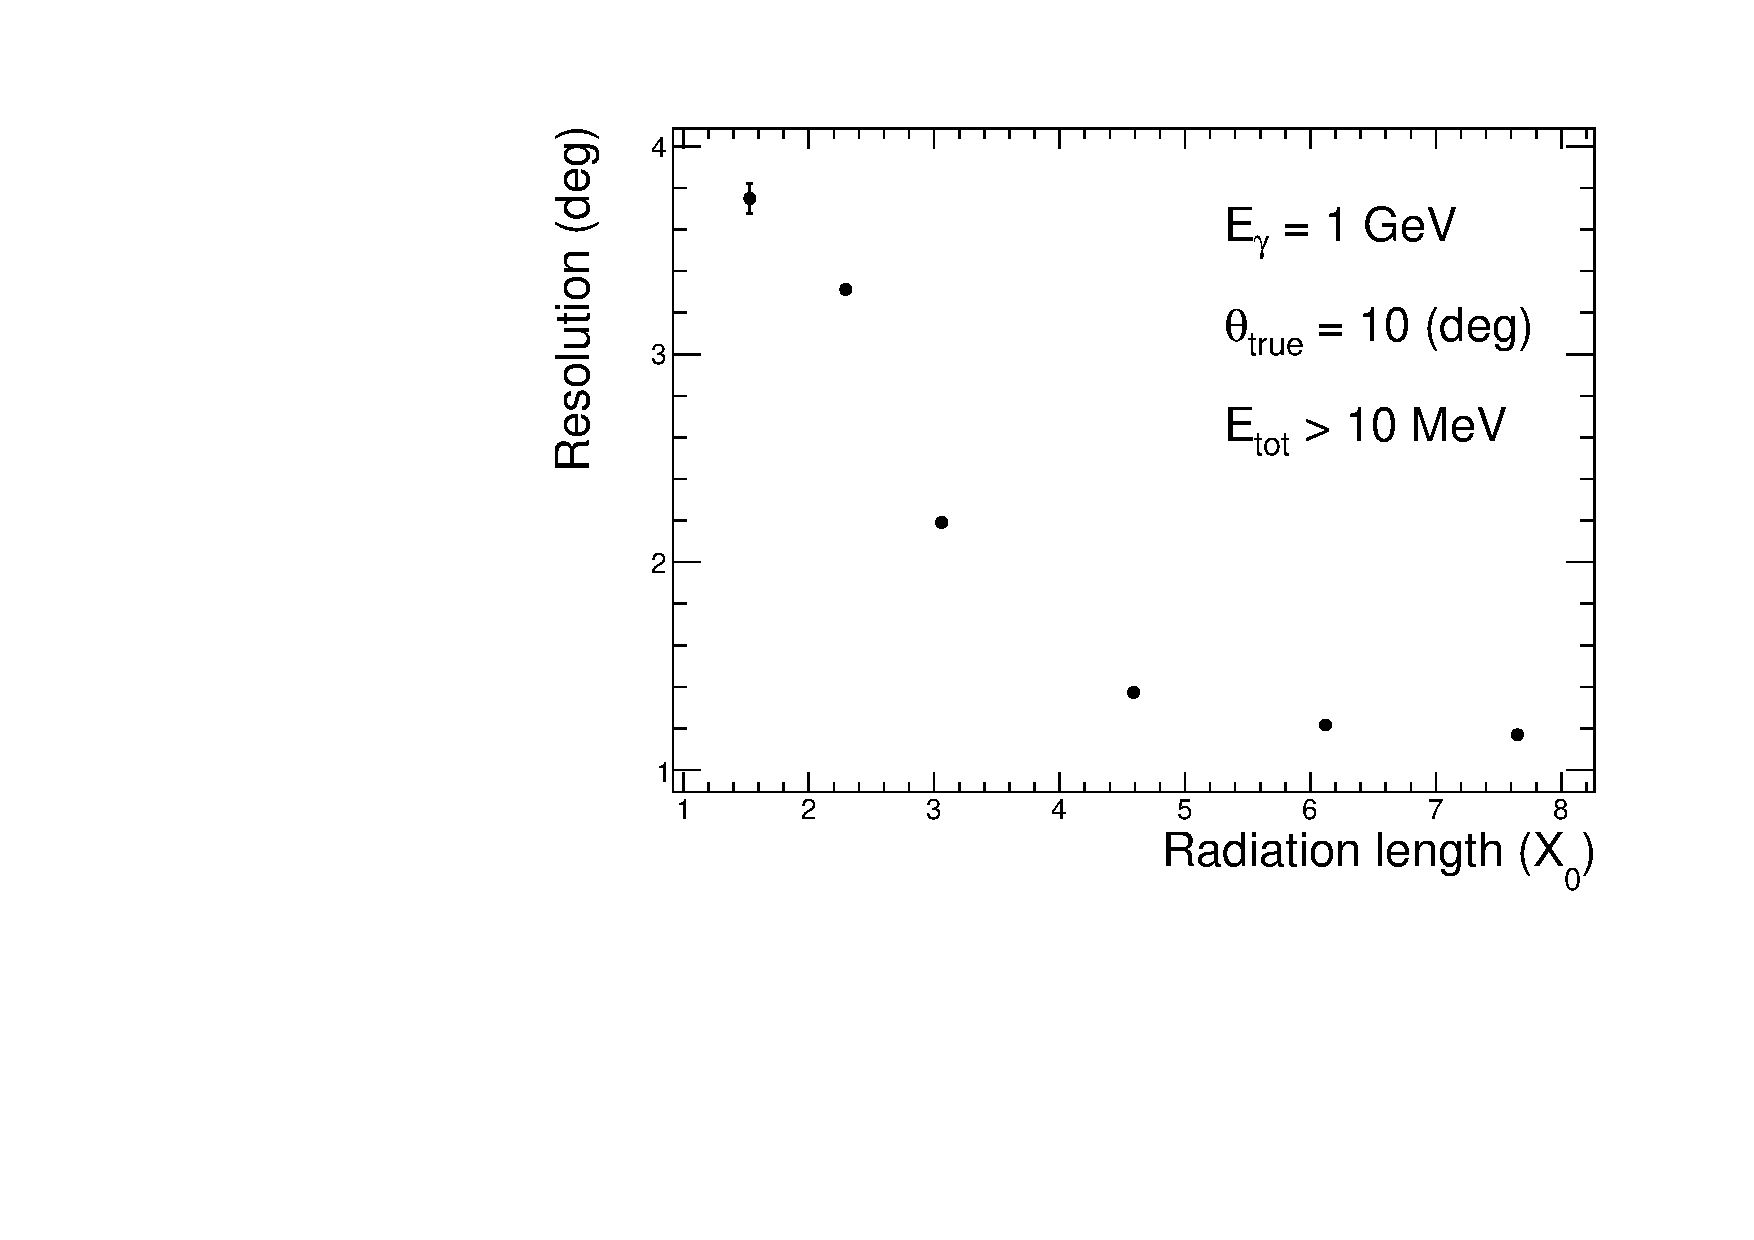
\includegraphics[width=0.48\textwidth]{figures/Fig3_reco_layer_graph.pdf}
\caption{ (Color online) Reconstructed $\theta$ for 1 GeV and $\theta_{\rm{true}}=$~10~deg $\gamma$ with (red) and without (black) the total energy ($E_{\rm{tot}}$) selection (left), and the angular resolution as a function of front layer depth used for the reconstruction (right). The inefficiency for 4.6$X_{0}$ is estimated to be 5.8\%  }
\label{fig:angle_reco_layer}
\end{figure}

The angle reconstruction is tested only with signals in front layers. Usages of front-layer signals are applied to the data sample for training and test procedures at the same time. The reconstruction with 24 layers, which possess the 4.6$X_{0}$, provides the identical resolution with one from full geometry. The inefficiency can arise mainly due to no responses in the front region, and can be evaluated by comparing the number of events with and without applying the minimum total energy ($E_{\rm{tot}}$) threshold in the front region. The inefficiency for (4.6$X_{0}$) is estimated to be 5.8\%. Figure~\ref{fig:angle_reco_layer} shows the reconstructed $\theta$ distribution (left) and the angular resolution as a function of front layer depth used for the reconstruction (right). The reconstructed $\theta$ without the $E_{\rm{tot}}$ threshold exhibits a delta peak near $\theta=$~0 as a results of not enough information to reconstruct $\theta$, And this peak clearly disappears by applying the $E_{\rm{tot}}$ threshold. The angular resolution is evaluated after applying the $E_{\rm{tot}}$ threshold and estimated to be 1.3 deg, which is comparable results with fig.~\ref{fig:angle_reco_width} for 4.6$X_{0}$ depth, so that the radiation length for the $\theta$ reconstruction is determined to be 4.6$X_{0}$.



The energy threshold and the attenuation effects are studied. The attenuation effect is applied to the deposit energies in each channel with the attenuation function~\cite{Murayama:2020mcp}. The energy threshold is applied to the all channels after the application of the attenuation effect. The coefficients of the attenuation effect are thought to be same as~\cite{Murayama:2020mcp}, and the applied threshold is 0.5~MeV. These responses are applied to the data sample for the training and test procedure. The angular resolution is found to be consistent with the resolution without such effects.



The incident angle and the incident energy dependencies of the angle reconstruction are studied with the same configuration and requirements mentioned before. It is found that 




\section{Conclusions}

\label{sec:con}


%\pagebreak

\begin{acknowledgments}
\end{acknowledgments}

\bibliography{paper}

\end{document}
